\documentclass[12pt,a4paper]{article}

% ============================================================
% PACKAGES
% ============================================================
\usepackage[utf8]{inputenc}
\usepackage[T1]{fontenc}
\usepackage{geometry}
\geometry{margin=2.5cm}

\usepackage{graphicx}
\usepackage{xcolor}
\usepackage{listings}
\usepackage{booktabs}
\usepackage{array}
\usepackage{tabularx}
\usepackage{enumitem}
\usepackage{tikz}
\usetikzlibrary{shapes.geometric, arrows.meta, positioning, calc}
\usepackage[hidelinks]{hyperref}
\usepackage{fancyhdr}
\usepackage{tcolorbox}
\tcbuselibrary{skins, breakable}
\usepackage{lmodern}

% ============================================================
% COLORS
% ============================================================
\definecolor{codeblue}{RGB}{0, 102, 204}
\definecolor{codegray}{RGB}{100, 100, 100}
\definecolor{codegreen}{RGB}{34, 139, 34}
\definecolor{codebg}{RGB}{245, 245, 245}
\definecolor{warnorange}{RGB}{230, 126, 34}
\definecolor{notblue}{RGB}{41, 128, 185}
\definecolor{impred}{RGB}{192, 57, 43}
\definecolor{tipgreen}{RGB}{39, 174, 96}
\definecolor{darkblue}{RGB}{26, 54, 93}

% ============================================================
% CODE LISTING STYLE
% ============================================================
\lstdefinestyle{cstyle}{
    language=C,
    backgroundcolor=\color{codebg},
    basicstyle=\ttfamily\small,
    keywordstyle=\color{codeblue}\bfseries,
    commentstyle=\color{codegreen}\itshape,
    stringstyle=\color{impred},
    numberstyle=\tiny\color{codegray},
    numbers=left,
    numbersep=8pt,
    frame=single,
    rulecolor=\color{codegray!30},
    breaklines=true,
    tabsize=4,
    showstringspaces=false,
    columns=flexible,
    morekeywords={BOOL, DWORD, HANDLE, LPCSTR, LPSTR, LPSTARTUPINFO,
                  LPPROCESS_INFORMATION, WINAPI, STARTUPINFO,
                  PROCESS_INFORMATION, SYSTEMTIME, TRUE, FALSE,
                  INFINITE, CTRL_C_EVENT, WAIT_OBJECT_0,
                  volatile, NULL, CREATE_SUSPENDED}
}
\lstset{style=cstyle}

\lstdefinestyle{pseudostyle}{
    backgroundcolor=\color{codebg},
    basicstyle=\ttfamily\small,
    frame=single,
    rulecolor=\color{codegray!30},
    breaklines=true,
    numbers=left,
    numberstyle=\tiny\color{codegray},
    numbersep=8pt,
}

% ============================================================
% TCOLORBOX STYLES
% ============================================================
\newtcolorbox{notebox}[1][]{
    enhanced, breakable,
    colback=notblue!5, colframe=notblue!80,
    fonttitle=\bfseries, title={\small Note}, #1
}

\newtcolorbox{importantbox}[1][]{
    enhanced, breakable,
    colback=impred!5, colframe=impred!80,
    fonttitle=\bfseries, title={\small Important}, #1
}

\newtcolorbox{warningbox}[1][]{
    enhanced, breakable,
    colback=warnorange!5, colframe=warnorange!80,
    fonttitle=\bfseries, title={\small Warning}, #1
}

\newtcolorbox{tipbox}[1][]{
    enhanced, breakable,
    colback=tipgreen!5, colframe=tipgreen!80,
    fonttitle=\bfseries, title={\small Tip}, #1
}

% ============================================================
% TIKZ STYLES
% ============================================================
\tikzset{
    proc/.style={rectangle, rounded corners=4pt, minimum width=3.2cm,
                 minimum height=0.9cm, text centered, draw=darkblue!60,
                 fill=blue!8, font=\small, text width=3.5cm,
                 line width=0.6pt},
    deci/.style={diamond, minimum width=2cm, minimum height=1cm,
                 text centered, draw=warnorange!70, fill=yellow!10,
                 font=\small, aspect=2.5, inner sep=1pt,
                 line width=0.6pt},
    startstop/.style={rectangle, rounded corners=4pt, minimum width=2.5cm,
                      minimum height=0.8cm, text centered, draw=impred!60,
                      fill=red!8, font=\small, line width=0.6pt},
    arr/.style={thick, -Stealth, color=codegray},
    participant/.style={rectangle, draw=darkblue!60, minimum width=2.5cm,
                        minimum height=0.7cm, fill=#1, font=\small\bfseries,
                        text centered, line width=0.6pt},
}

% ============================================================
% HEADER / FOOTER
% ============================================================
\pagestyle{fancy}
\fancyhf{}
\fancyhead[L]{\small\textit{myShell}}
\fancyhead[R]{\small\thepage}
\fancyfoot[C]{\small Operating Systems --- HUST}
\renewcommand{\headrulewidth}{0.4pt}

% ============================================================
% DOCUMENT
% ============================================================
\begin{document}

% ---- TITLE ----
\begin{center}
    {\color{darkblue}\LARGE\bfseries How a Shell Works}\\[0.2cm]
    \begin{tabular}{rl}
        \textbf{Project:} & Tiny Shell (myShell) \\
        \textbf{Author :} & Pham Van Sam \\ 
        \textbf{ID student :} & 202400114 \\ 
        \textbf{Course:} & Operating Systems \\
        \textbf{University:} & Hanoi University of Science and Technology \\
    \end{tabular}
\end{center}

\tableofcontents
\newpage

% ============================================================
% SECTION 1
% ============================================================
\section{What is a Shell?}

A shell is a \textbf{command-line interface} (CLI) program that acts as an \textbf{intermediary} between the user and the operating system. When you type a command such as \texttt{notepad hello.txt}, the shell performs the following sequence of operations:

\begin{enumerate}
    \item \textbf{Read} the string of characters you entered.
    \item \textbf{Parse} it to determine which program to run and with what arguments.
    \item \textbf{Request} the OS to create a new child process to execute that program.
    \item \textbf{Wait} (or not) for the child process to terminate.
    \item \textbf{Return} to the prompt and wait for the next command.
\end{enumerate}

In essence, a shell is nothing more than an infinite loop that reads, evaluates, and prints --- commonly referred to as a \textbf{REPL} (Read-Eval-Print Loop).

% ============================================================
% SECTION 2
% ============================================================
\section{The Main Loop --- Heart of Every Shell}

\begin{importantbox}
    The \textbf{REPL loop} is the single most important concept. Every shell, from \texttt{cmd.exe} to \texttt{bash} to our \texttt{myShell}, is built around this loop. If you understand this, you understand the entire program.
\end{importantbox}

\begin{center}
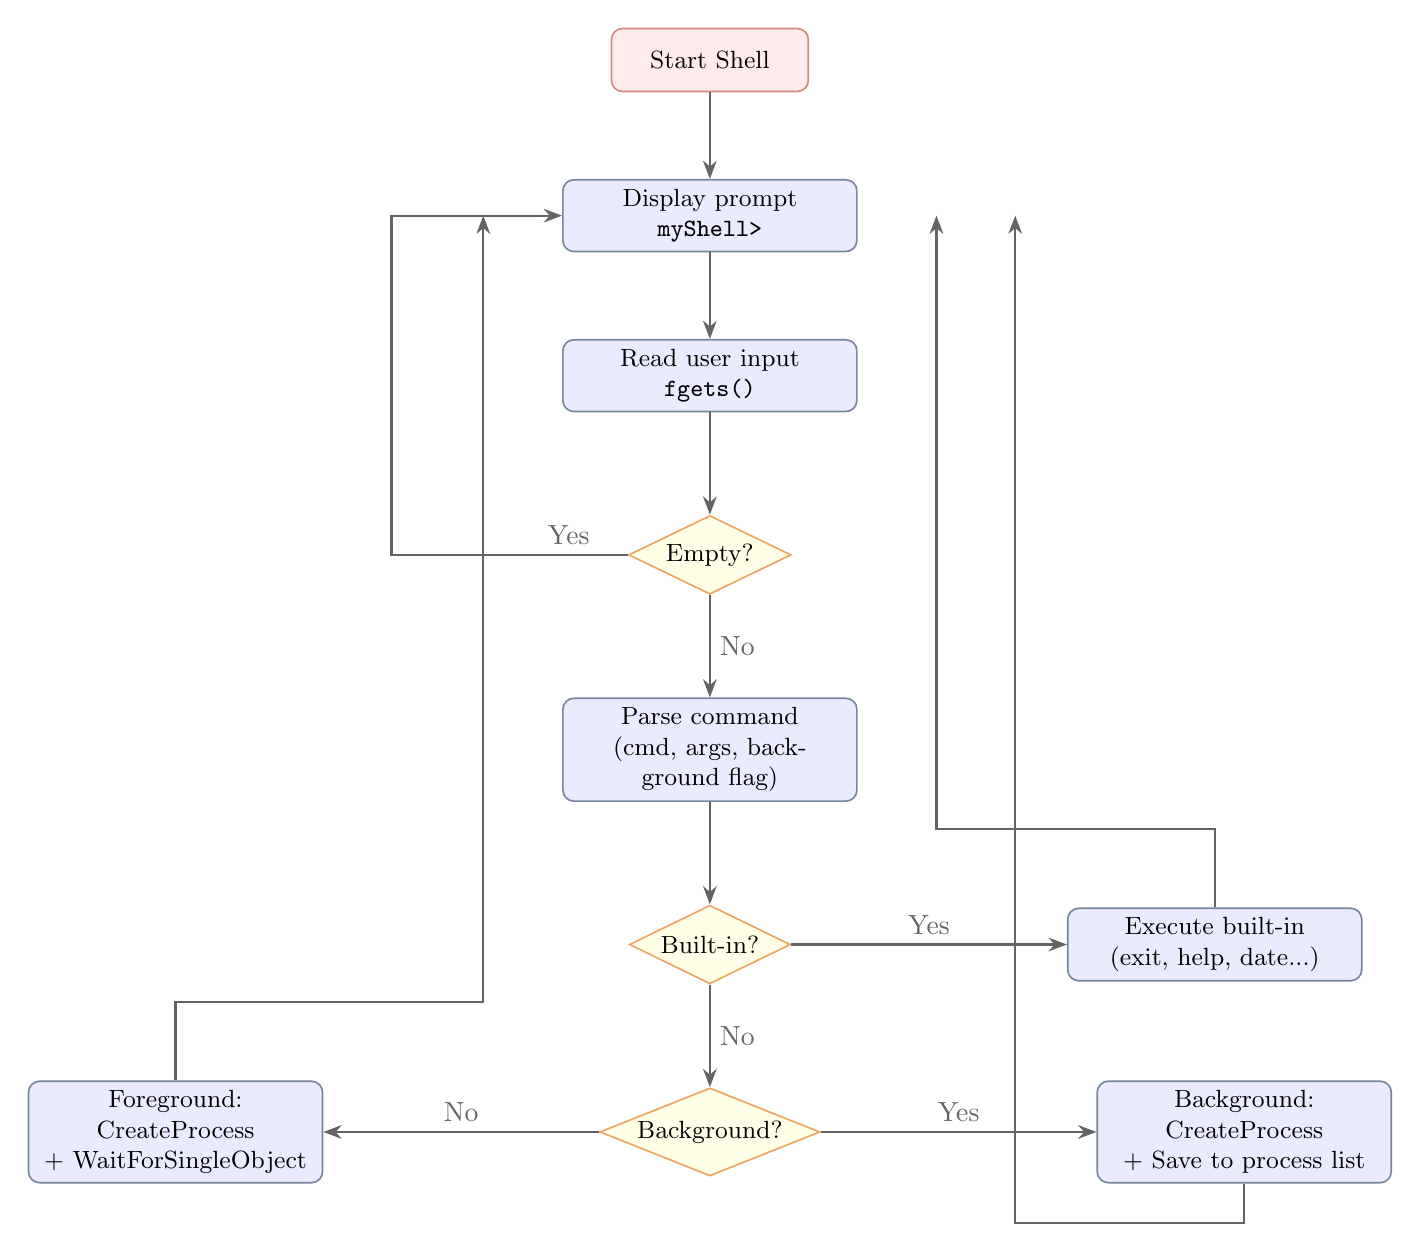
\begin{tikzpicture}[node distance=1.1cm, auto]
    \node[startstop] (start) {Start Shell};
    \node[proc, below=of start] (prompt) {Display prompt\\{\ttfamily myShell>}};
    \node[proc, below=of prompt] (read) {Read user input\\{\ttfamily fgets()}};
    \node[deci, below=1.3cm of read] (empty) {Empty?};
    \node[proc, below=1.3cm of empty] (parse) {Parse command\\(cmd, args, background flag)};
    \node[deci, below=1.3cm of parse] (builtin) {Built-in?};
    \node[proc, right=3.5cm of builtin] (execbi) {Execute built-in\\(exit, help, date...)};
    \node[deci, below=1.3cm of builtin] (bgcheck) {Background?};
    \node[proc, left=3.5cm of bgcheck] (fg) {Foreground:\\CreateProcess\\+ WaitForSingleObject};
    \node[proc, right=3.5cm of bgcheck] (bg) {Background:\\CreateProcess\\+ Save to process list};

    \draw[arr] (start) -- (prompt);
    \draw[arr] (prompt) -- (read);
    \draw[arr] (read) -- (empty);
    \draw[arr] (empty) -- node[right] {No} (parse);
    \draw[arr] (empty.west) -- ++(-3,0) node[above, near start] {Yes} |- (prompt.west);
    \draw[arr] (parse) -- (builtin);
    \draw[arr] (builtin) -- node[above] {Yes} (execbi);
    \draw[arr] (execbi.north) -- ++(0,1) -| ([xshift=1cm]prompt.east);
    \draw[arr] (builtin) -- node[right] {No} (bgcheck);
    \draw[arr] (bgcheck) -- node[above] {No} (fg);
    \draw[arr] (bgcheck) -- node[above] {Yes} (bg);
    \draw[arr] (fg.north) -- ++(0,1) -| ([xshift=-1cm]prompt.west);
    \draw[arr] (bg.south) -- ++(0,-0.5) -| ([xshift=2cm]prompt.east);
\end{tikzpicture}
\end{center}

% ============================================================
% SECTION 3
% ============================================================
\section{Parsing --- How the Shell Understands You}

When the user types: \texttt{notepad hello.txt \&}

The parser must decompose this into three distinct pieces of information:

\begin{center}
\begin{tabular}{lll}
    \toprule
    \textbf{Component} & \textbf{Value} & \textbf{Meaning} \\
    \midrule
    Command & \texttt{notepad} & The program to execute \\
    Arguments & \texttt{hello.txt} & Parameters passed to the program \\
    Background flag & \texttt{\&} & Run concurrently with the shell \\
    \bottomrule
\end{tabular}
\end{center}

\subsection{Parsing Algorithm}

\begin{lstlisting}[style=pseudostyle]
1. Read the entire input line
2. Strip the trailing newline '\n'
3. Check if the last non-space character is '&'
   -> If yes: set isBackground = true, remove '&'
   -> If no:  set isBackground = false
4. Tokenize by spaces using strtok()
   -> First token  = command name
   -> Remaining tokens = arguments
5. Concatenate into a full command line for CreateProcess()
\end{lstlisting}

\begin{notebox}
    Unlike Unix, where \texttt{execvp()} takes an array of arguments, the Windows API \texttt{CreateProcess()} expects the \textbf{entire command line as a single string} (e.g., \texttt{"notepad hello.txt"}). However, you still need to extract the command name separately to check whether it is a built-in command.
\end{notebox}

% ============================================================
% SECTION 4
% ============================================================
\section{Executing Commands --- CreateProcess() in Depth}

\subsection{What is CreateProcess()?}

\texttt{CreateProcess()} is the fundamental Windows API for \textbf{spawning a new child process}. Its simplified signature:

\begin{lstlisting}
BOOL CreateProcess(
    LPCSTR lpApplicationName,    // Path to .exe (can be NULL)
    LPSTR  lpCommandLine,        // Full command line string
    ...                          // Security, inheritance, etc.
    BOOL   bInheritHandles,      // Inherit parent handles?
    DWORD  dwCreationFlags,      // Flags (0, CREATE_SUSPENDED, ...)
    ...
    LPSTARTUPINFO lpStartupInfo,         // Startup configuration
    LPPROCESS_INFORMATION lpProcessInfo  // [OUT] PID, handles
);
\end{lstlisting}

\subsection{The Process Creation Timeline}

The following diagram illustrates the sequence of events when the shell creates and manages a foreground process:

\begin{center}
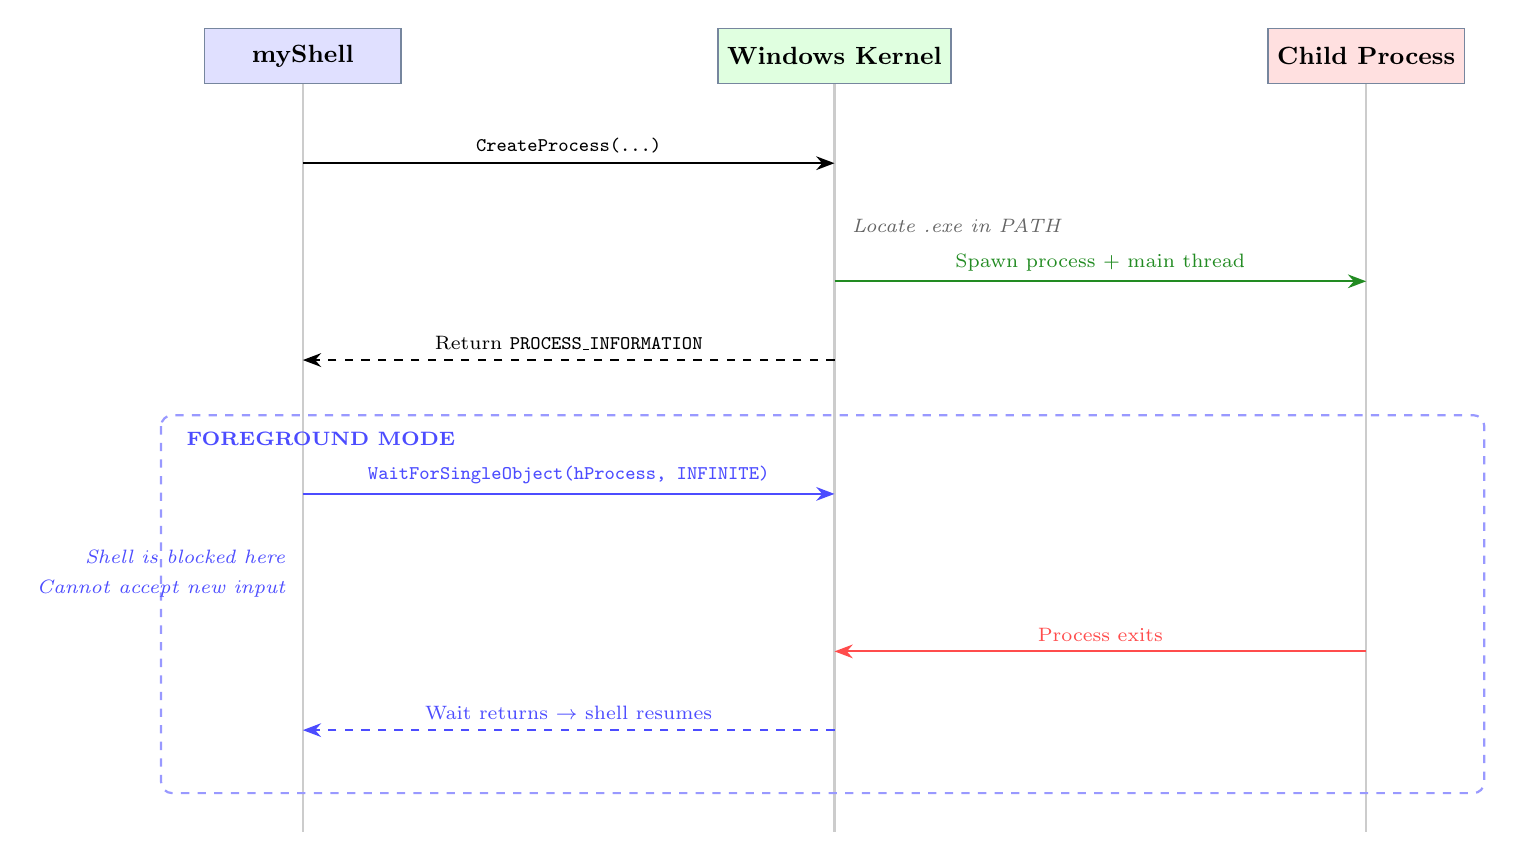
\begin{tikzpicture}[
    arr/.style={-Stealth, thick},
    darr/.style={-Stealth, thick, dashed},
]
    % Participants
    \node[participant=blue!12] (shell) {myShell};
    \node[participant=green!12, right=4cm of shell] (os) {Windows Kernel};
    \node[participant=red!12, right=4cm of os] (child) {Child Process};

    % Lifelines
    \draw[thick, gray!40] (shell.south) -- ++(0,-9.5);
    \draw[thick, gray!40] (os.south) -- ++(0,-9.5);
    \draw[thick, gray!40] (child.south) -- ++(0,-9.5);

    % Step 1
    \draw[arr] ($(shell.south)+(0,-1)$) -- ($(os.south)+(0,-1)$)
        node[midway, above, font=\scriptsize] {\texttt{CreateProcess(...)}};

    % Step 2
    \node[font=\scriptsize\itshape\color{codegray}, right]
        at ($(os.south)+(0.1,-1.8)$) {Locate .exe in PATH};

    % Step 3
    \draw[arr, codegreen] ($(os.south)+(0,-2.5)$) -- ($(child.south)+(0,-2.5)$)
        node[midway, above, font=\scriptsize] {Spawn process + main thread};

    % Step 4
    \draw[darr] ($(os.south)+(0,-3.5)$) -- ($(shell.south)+(0,-3.5)$)
        node[midway, above, font=\scriptsize] {Return \texttt{PROCESS\_INFORMATION}};

    % Foreground box
    \draw[thick, blue!40, rounded corners, dashed]
        ($(shell.south)+(-1.8,-4.2)$) rectangle ($(child.south)+(1.5,-9)$);
    \node[font=\scriptsize\bfseries\color{blue!70}, anchor=west]
        at ($(shell.south)+(-1.6,-4.5)$) {FOREGROUND MODE};

    % Step 5
    \draw[arr, blue!70] ($(shell.south)+(0,-5.2)$) -- ($(os.south)+(0,-5.2)$)
        node[midway, above, font=\scriptsize\color{blue!70}]
        {\texttt{WaitForSingleObject(hProcess, INFINITE)}};

    % Blocked note
    \node[font=\scriptsize\itshape\color{blue!70}, anchor=east]
        at ($(shell.south)+(-0.1,-6)$) {Shell is blocked here};
    \node[font=\scriptsize\itshape\color{blue!70}, anchor=east]
        at ($(shell.south)+(-0.1,-6.4)$) {Cannot accept new input};

    % Step 6
    \draw[arr, red!70] ($(child.south)+(0,-7.2)$) -- ($(os.south)+(0,-7.2)$)
        node[midway, above, font=\scriptsize\color{red!70}] {Process exits};

    % Step 7
    \draw[darr, blue!70] ($(os.south)+(0,-8.2)$) -- ($(shell.south)+(0,-8.2)$)
        node[midway, above, font=\scriptsize\color{blue!70}]
        {Wait returns $\rightarrow$ shell resumes};
\end{tikzpicture}
\end{center}

\subsection{The PROCESS\_INFORMATION Structure}

Upon success, \texttt{CreateProcess()} populates this output structure:

\begin{lstlisting}
typedef struct {
    HANDLE hProcess;    // Handle to the child process (for Wait, Kill)
    HANDLE hThread;     // Handle to the main thread (for Suspend/Resume)
    DWORD  dwProcessId; // Process ID (e.g., 12345)
    DWORD  dwThreadId;  // Thread ID of the main thread
} PROCESS_INFORMATION;
\end{lstlisting}

\begin{warningbox}
    You \textbf{must store both} \texttt{hProcess} and \texttt{hThread} for background processes.
    \begin{itemize}[nosep]
        \item \texttt{hProcess} is used for \texttt{TerminateProcess()} and \texttt{WaitForSingleObject()}.
        \item \texttt{hThread} is used for \texttt{SuspendThread()} and \texttt{ResumeThread()}.
    \end{itemize}
    Forgetting to call \texttt{CloseHandle()} when a process terminates causes a \textbf{handle leak} (similar to a memory leak).
\end{warningbox}

% ============================================================
% SECTION 5
% ============================================================
\section{Foreground vs.\ Background Execution}

The only difference between the two modes is a single line of code: \texttt{WaitForSingleObject()}. Everything else is identical.

\begin{center}
\renewcommand{\arraystretch}{1.3}
\begin{tabularx}{\textwidth}{l X X}
    \toprule
     & \textbf{Foreground} & \textbf{Background} \\
    \midrule
    \textbf{Syntax} & \texttt{notepad hello.txt} & \texttt{notepad hello.txt \&} \\
    \textbf{Shell blocked?} & Yes --- waits via \texttt{WaitForSingleObject()} & No --- returns to prompt immediately \\
    \textbf{User experience} & Cannot type until process finishes & Can type new commands right away \\
    \textbf{Handle lifecycle} & \texttt{CloseHandle()} immediately after Wait & Store in list; \texttt{CloseHandle()} on kill or natural exit \\
    \bottomrule
\end{tabularx}
\end{center}

\subsection{Side-by-Side Code Comparison}

\begin{lstlisting}
CreateProcess(NULL, commandLine, NULL, NULL, FALSE, 0,
              NULL, NULL, &si, &pi);

if (isBackground) {
    // --- BACKGROUND MODE ---
    // Do NOT wait. Save process info for later management.
    addToProcessList(pi, commandName);
    printf("[%d] %s\n", pi.dwProcessId, commandName);
    // Do NOT close handles here --- we need them later.
} else {
    // --- FOREGROUND MODE ---
    // Block the shell until the child process terminates.
    WaitForSingleObject(pi.hProcess, INFINITE);
    // Child is done --- clean up handles.
    CloseHandle(pi.hProcess);
    CloseHandle(pi.hThread);
}
\end{lstlisting}

% ============================================================
% SECTION 6
% ============================================================
\section{Background Process Management}

\subsection{Data Structure}

We maintain a simple array of structs to track all background processes:

\begin{lstlisting}
#define MAX_BG 100

typedef struct {
    DWORD   pid;           // Process ID
    HANDLE  hProcess;      // Process handle (for Kill, Wait)
    HANDLE  hThread;       // Thread handle (for Suspend, Resume)
    char    cmdName[256];  // Original command name
    int     status;        // RUNNING | STOPPED | TERMINATED
} BackgroundProcess;

BackgroundProcess bgProcesses[MAX_BG];
int bgCount = 0;
\end{lstlisting}

\subsection{Management Commands and Their APIs}

\begin{center}
\renewcommand{\arraystretch}{1.3}
\begin{tabularx}{\textwidth}{l l X}
    \toprule
    \textbf{Shell Command} & \textbf{Windows API} & \textbf{Description} \\
    \midrule
    \texttt{list} & \texttt{WaitForSingleObject(h, 0)} & Iterate through array, print PID, name, and status. Use a zero timeout to poll whether each process is still alive without blocking. \\
    \texttt{kill <pid>} & \texttt{TerminateProcess(h, 0)} & Forcefully terminate the process. No cleanup occurs in the child. \\
    \texttt{stop <pid>} & \texttt{SuspendThread(hThread)} & Suspend the main thread. The process remains in memory but does not execute. \\
    \texttt{resume <pid>} & \texttt{ResumeThread(hThread)} & Resume a previously suspended thread. \\
    \bottomrule
\end{tabularx}
\end{center}

\begin{tipbox}
    When implementing \texttt{list}, call \texttt{WaitForSingleObject(hProcess, 0)} for each process. If it returns \texttt{WAIT\_OBJECT\_0}, the process has already terminated naturally. In that case, update its status to \texttt{TERMINATED} and call \texttt{CloseHandle()} to release the kernel resources.
\end{tipbox}

% ============================================================
% SECTION 7
% ============================================================
\section{Built-in Commands --- Executed Inside the Shell}

Built-in commands are handled \textbf{directly within the shell process itself}, without spawning a child process.

\begin{center}
\renewcommand{\arraystretch}{1.3}
\begin{tabularx}{\textwidth}{l X}
    \toprule
    \textbf{Command} & \textbf{Implementation} \\
    \midrule
    \texttt{exit} & Break the main loop $\rightarrow$ terminate the shell \\
    \texttt{help} & Print a usage guide listing all available commands \\
    \texttt{date} & Call \texttt{GetLocalTime()} $\rightarrow$ print the current date \\
    \texttt{time} & Call \texttt{GetLocalTime()} $\rightarrow$ print the current time \\
    \texttt{dir} & List files via \texttt{FindFirstFile()} + \texttt{FindNextFile()} \\
    \texttt{path} & Call \texttt{GetEnvironmentVariable("PATH", ...)} and print the result \\
    \texttt{addpath <p>} & Read the current PATH, append \texttt{;<p>}, then call \texttt{SetEnvironmentVariable("PATH", ...)} \\
    \bottomrule
\end{tabularx}
\end{center}

\subsection{Why Must These Be Built-in?}

\begin{itemize}
    \item \texttt{exit} must run inside the shell process. You cannot spawn a child process to terminate the parent --- the parent would simply continue running.
    \item \texttt{addpath} modifies the shell's own environment variables. On Windows (and Unix), each process has its own \textbf{private copy} of the environment. If \texttt{addpath} ran in a child process, the modification would vanish when the child exits, leaving the parent's PATH unchanged.
\end{itemize}

% ============================================================
% SECTION 8
% ============================================================
\section{Handling CTRL+C --- Graceful Signal Management}

\subsection{The Problem}

By default, when the user presses CTRL+C, Windows sends a \texttt{CTRL\_C\_EVENT} to \textbf{all processes} attached to the same console --- both the shell and any running child process. Without intervention, the shell itself would terminate.

\subsection{The Solution}

Register a custom handler using \texttt{SetConsoleCtrlHandler()} that intercepts the signal:

\begin{center}
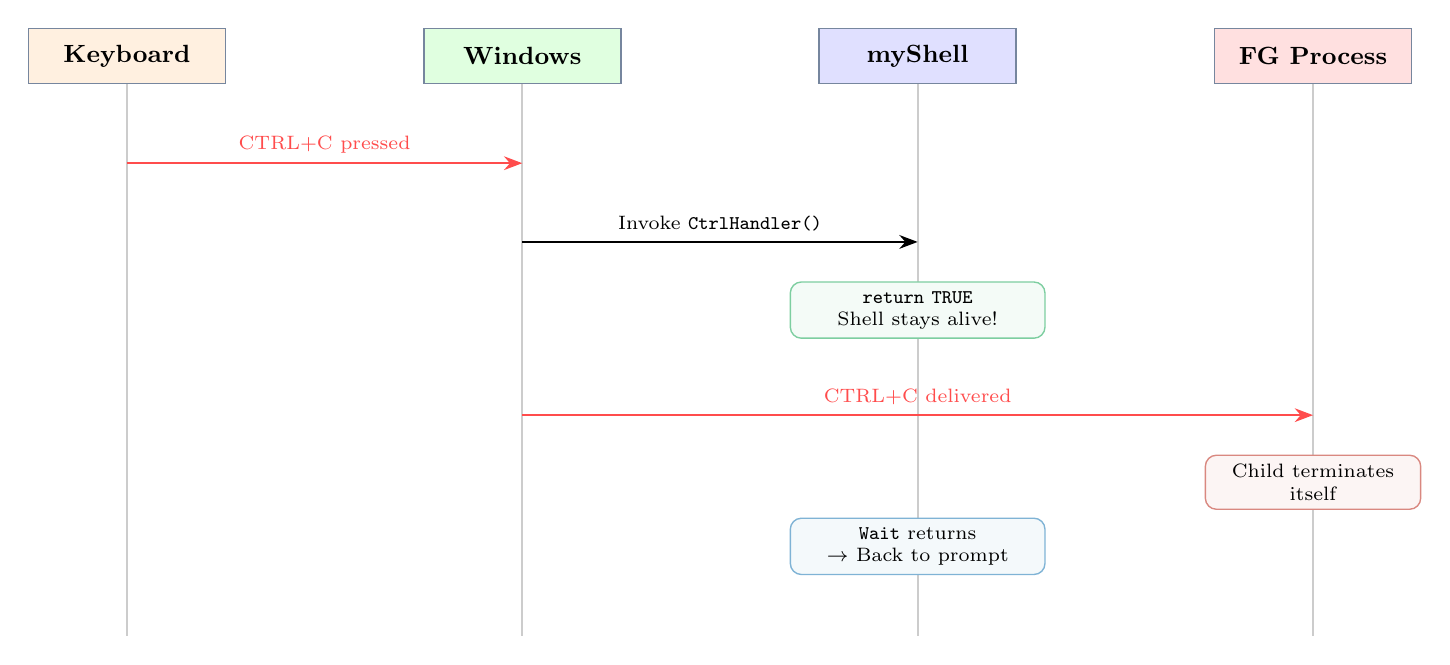
\begin{tikzpicture}[
    arr/.style={-Stealth, thick},
]
    % Participants
    \node[participant=orange!12] (user) {Keyboard};
    \node[participant=green!12, right=2.5cm of user] (os) {Windows};
    \node[participant=blue!12, right=2.5cm of os] (shell) {myShell};
    \node[participant=red!12, right=2.5cm of shell] (fg) {FG Process};

    % Lifelines
    \draw[thick, gray!40] (user.south) -- ++(0,-7);
    \draw[thick, gray!40] (os.south) -- ++(0,-7);
    \draw[thick, gray!40] (shell.south) -- ++(0,-7);
    \draw[thick, gray!40] (fg.south) -- ++(0,-7);

    % CTRL+C
    \draw[arr, red!70] ($(user.south)+(0,-1)$) -- ($(os.south)+(0,-1)$)
        node[midway, above, font=\scriptsize] {CTRL+C pressed};

    % OS dispatches to shell handler
    \draw[arr] ($(os.south)+(0,-2)$) -- ($(shell.south)+(0,-2)$)
        node[midway, above, font=\scriptsize] {Invoke \texttt{CtrlHandler()}};

    % Shell note
    \node[rectangle, rounded corners, draw=tipgreen!60, fill=tipgreen!5,
          font=\scriptsize, text width=3cm, align=center,
          anchor=north, line width=0.5pt]
        at ($(shell.south)+(0,-2.5)$)
        {\texttt{return TRUE}\\Shell stays alive!};

    % OS also sends to child
    \draw[arr, red!70] ($(os.south)+(0,-4.2)$) -- ($(fg.south)+(0,-4.2)$)
        node[midway, above, font=\scriptsize] {CTRL+C delivered};

    % Child terminates
    \node[rectangle, rounded corners, draw=impred!60, fill=impred!5,
          font=\scriptsize, text width=2.5cm, align=center,
          anchor=north, line width=0.5pt]
        at ($(fg.south)+(0,-4.7)$)
        {Child terminates\\itself};

    % Shell resumes
    \node[rectangle, rounded corners, draw=notblue!60, fill=notblue!5,
          font=\scriptsize, text width=3cm, align=center,
          anchor=north, line width=0.5pt]
        at ($(shell.south)+(0,-5.5)$)
        {\texttt{Wait} returns\\$\rightarrow$ Back to prompt};
\end{tikzpicture}
\end{center}

\subsection{Implementation}

\begin{lstlisting}
// Global flag: is there a foreground process running?
volatile BOOL isRunningForeground = FALSE;

BOOL WINAPI CtrlHandler(DWORD ctrlType) {
    if (ctrlType == CTRL_C_EVENT) {
        if (isRunningForeground) {
            // The child process will receive CTRL+C from the OS
            // and terminate itself. We just need to survive.
            return TRUE;  // TRUE = "I handled it, don't kill me"
        }
        // No foreground process --- just reprint the prompt.
        printf("\nmyShell> ");
        return TRUE;
    }
    return FALSE;  // Let the OS handle other signals
}

// Register once at startup:
SetConsoleCtrlHandler(CtrlHandler, TRUE);
\end{lstlisting}

\begin{importantbox}
    Returning \texttt{TRUE} from the handler tells Windows: ``I have handled this signal; do not terminate my process.'' Returning \texttt{FALSE} causes the default behavior, which terminates the shell.
\end{importantbox}

% ============================================================
% SECTION 9
% ============================================================
\section{Executing Batch Files (.bat)}

A \texttt{.bat} file is not an executable --- it is a script interpreted by \texttt{cmd.exe}. On some Windows versions, calling \texttt{CreateProcess()} directly with a \texttt{.bat} file may fail. The reliable solution is to invoke the command interpreter explicitly:

\begin{lstlisting}
// When the command ends with ".bat":
char fullCmd[1024];
sprintf(fullCmd, "cmd.exe /c %s", originalCommandLine);
CreateProcess(NULL, fullCmd, NULL, NULL, FALSE, 0,
              NULL, NULL, &si, &pi);
\end{lstlisting}

Alternatively, you can \textbf{always pass \texttt{NULL}} as \texttt{lpApplicationName} and let Windows resolve the file type automatically:

\begin{lstlisting}
CreateProcess(
    NULL,           // Let Windows figure out the executable
    commandLine,    // "script.bat arg1 arg2"
    NULL, NULL, FALSE, 0, NULL, NULL, &si, &pi
);
// Windows detects the .bat extension and invokes cmd.exe internally
\end{lstlisting}

% ============================================================
% SECTION 10
% ============================================================
\section{Complete Execution Flow}

The following diagram summarizes the entire architecture of \texttt{myShell}, from initialization to shutdown:

\begin{center}
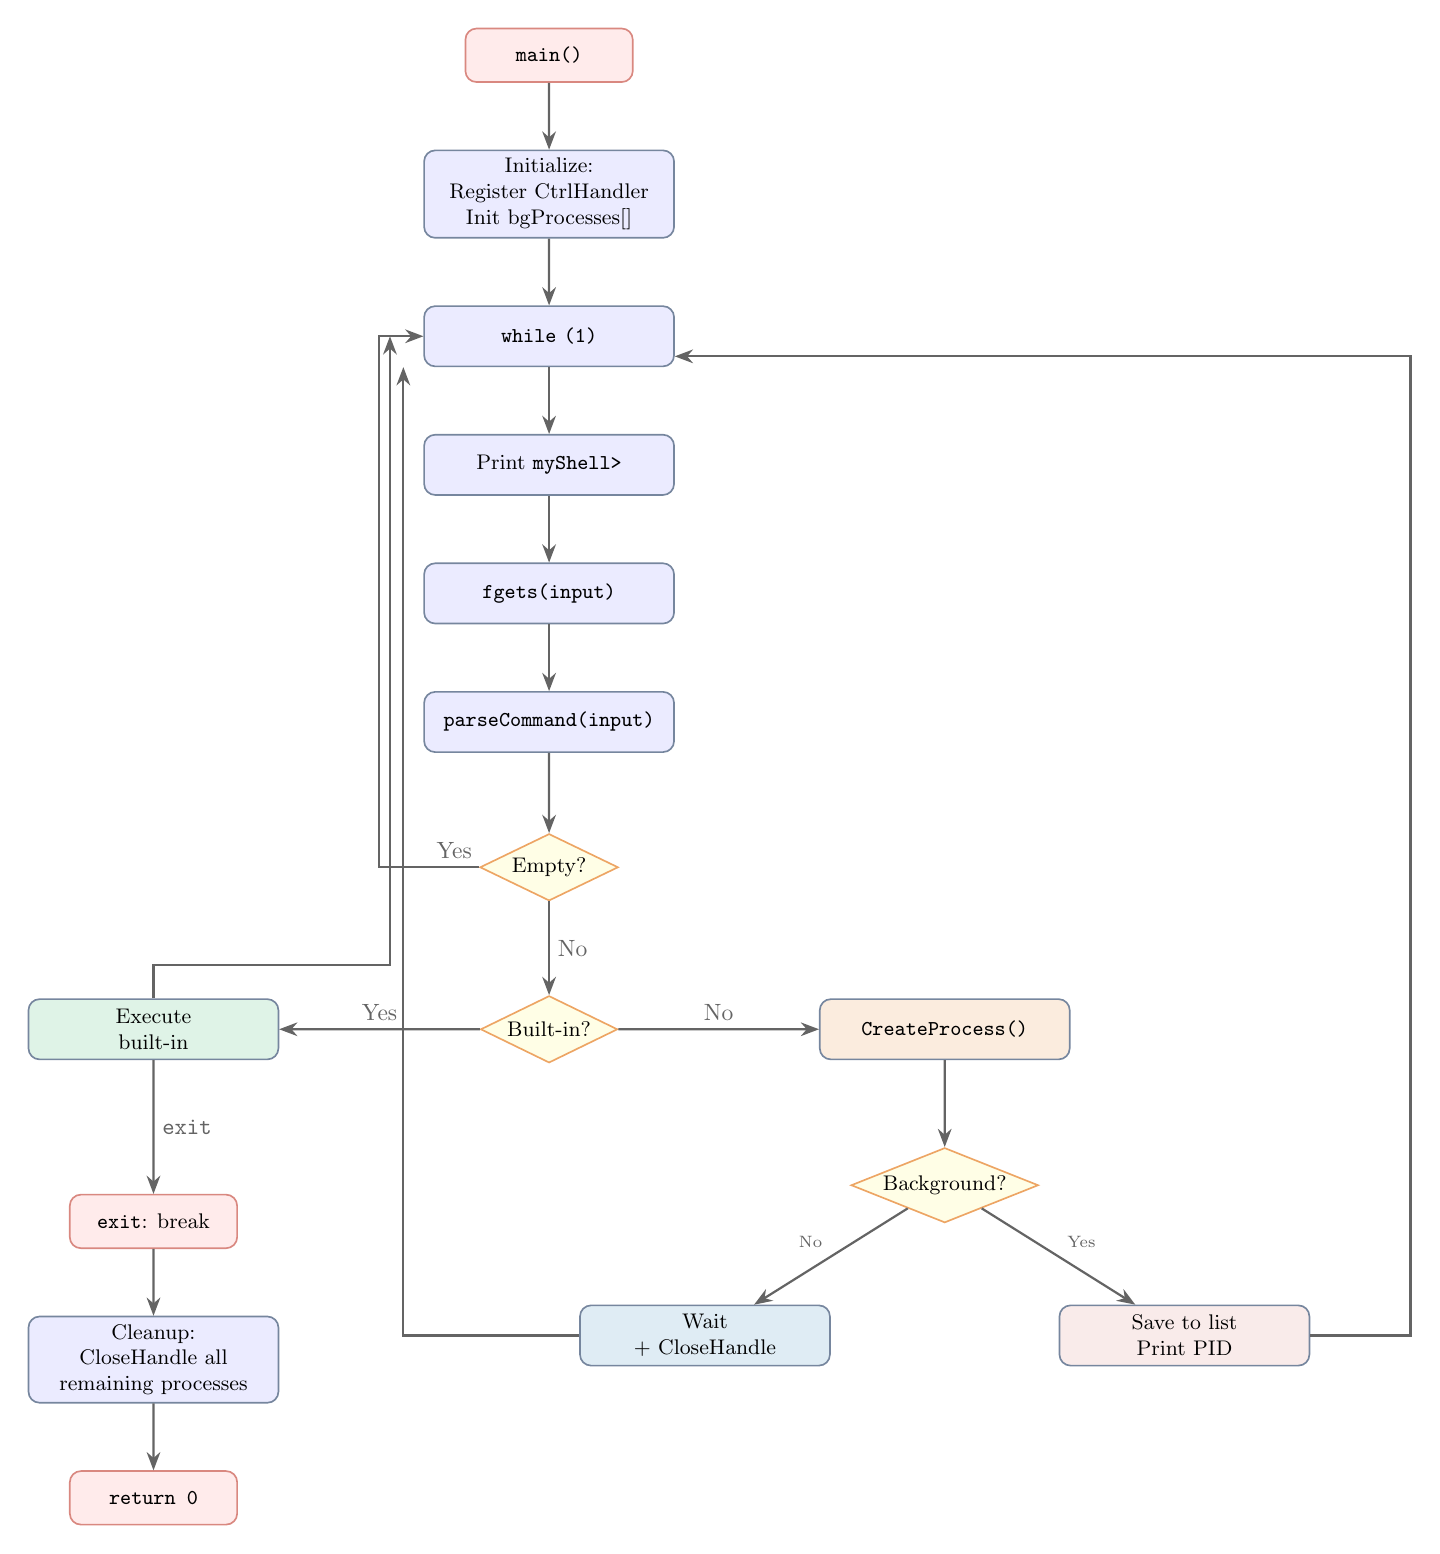
\begin{tikzpicture}[node distance=1cm, auto, scale=0.85, transform shape]
    \node[startstop] (start) {\texttt{main()}};
    \node[proc, below=of start] (init) {Initialize:\\Register CtrlHandler\\Init bgProcesses[]};
    \node[proc, below=of init] (loop) {\texttt{while (1)}};
    \node[proc, below=of loop] (prompt) {Print \texttt{myShell>}};
    \node[proc, below=of prompt] (read) {\texttt{fgets(input)}};
    \node[proc, below=of read] (parse) {\texttt{parseCommand(input)}};
    \node[deci, below=1.2cm of parse] (check) {Empty?};
    \node[deci, below=1.4cm of check] (bi) {Built-in?};

    % Left: built-in
    \node[proc, left=3cm of bi, fill=tipgreen!15] (execbi) {Execute\\built-in};
    \node[startstop, below=2cm of execbi] (exit) {\texttt{exit}: break};

    % Right: external
    \node[proc, right=3cm of bi, fill=warnorange!15] (external) {\texttt{CreateProcess()}};
    \node[deci, below=1.3cm of external] (bgq) {Background?};
    \node[proc, below left=1.5cm and 1cm of bgq, fill=notblue!15] (fgp) {Wait\\+ CloseHandle};
    \node[proc, below right=1.5cm and 1cm of bgq, fill=impred!10] (bgp) {Save to list\\Print PID};

    % Cleanup
    \node[proc, below=of exit] (cleanup) {Cleanup:\\CloseHandle all\\remaining processes};
    \node[startstop, below=of cleanup] (end) {\texttt{return 0}};

    % Main flow
    \draw[arr] (start) -- (init);
    \draw[arr] (init) -- (loop);
    \draw[arr] (loop) -- (prompt);
    \draw[arr] (prompt) -- (read);
    \draw[arr] (read) -- (parse);
    \draw[arr] (parse) -- (check);
    \draw[arr] (check) -- node[right] {No} (bi);
    \draw[arr] (check.west) -- ++(-1.5,0) node[above, near start] {Yes} |- (loop.west);

    % Built-in
    \draw[arr] (bi) -- node[above] {Yes} (execbi);
    \draw[arr] (execbi) -- node[right] {\texttt{exit}} (exit);
    \draw[arr] (execbi.north) -- ++(0,0.5) -| ([xshift=-0.5cm]loop.west);

    % External
    \draw[arr] (bi) -- node[above] {No} (external);
    \draw[arr] (external) -- (bgq);
    \draw[arr] (bgq) -- node[above left, font=\scriptsize] {No} (fgp);
    \draw[arr] (bgq) -- node[above right, font=\scriptsize] {Yes} (bgp);

    % Return to loop
    \draw[arr] (fgp.west) -| ([xshift=-0.3cm]loop.south west);
    \draw[arr] (bgp.east) -- ++(1.5,0) |- ([yshift=-0.3cm]loop.east);

    % Exit path
    \draw[arr] (exit) -- (cleanup);
    \draw[arr] (cleanup) -- (end);
\end{tikzpicture}
\end{center}

% ============================================================
% APPENDIX: Quick API Reference
% ============================================================
\newpage
\appendix
\section{Windows API Quick Reference}

\begin{center}
\renewcommand{\arraystretch}{1.4}
\begin{tabularx}{\textwidth}{l X}
    \toprule
    \textbf{API Function} & \textbf{Purpose in myShell} \\
    \midrule
    \texttt{CreateProcess()} & Spawn a new child process from a command line string \\
    \texttt{WaitForSingleObject()} & Block until a process terminates (foreground mode) \\
    \texttt{TerminateProcess()} & Forcefully kill a background process \\
    \texttt{SuspendThread()} & Pause a background process \\
    \texttt{ResumeThread()} & Resume a paused background process \\
    \texttt{CloseHandle()} & Release a kernel handle (process or thread) \\
    \texttt{SetConsoleCtrlHandler()} & Register a custom CTRL+C handler \\
    \texttt{GetLocalTime()} & Retrieve the current system date and time \\
    \texttt{GetEnvironmentVariable()} & Read an environment variable (e.g., PATH) \\
    \texttt{SetEnvironmentVariable()} & Modify an environment variable \\
    \texttt{FindFirstFile()} & Begin directory enumeration \\
    \texttt{FindNextFile()} & Continue directory enumeration \\
    \bottomrule
\end{tabularx}
\end{center}

\end{document}
